\chapter{Tables statistiques}
\newpage
%\section{Table de la loi binomiale avec $p$=0.5}
%\label{sec:tablebinomiale}
%\begin{center}
%\includegraphics[width=0.5\linewidth,clip]{table_bin_0_5}
%\end{center}

\section{Loi normale centr�e r�duite}
\label{sec:tablenormale}
% \newpage
% \section{Table de la loi normale centr�e-r�duite}
% \begin{center}
% \includegraphics[width=\linewidth,clip]{table_normale}
% \end{center}
$$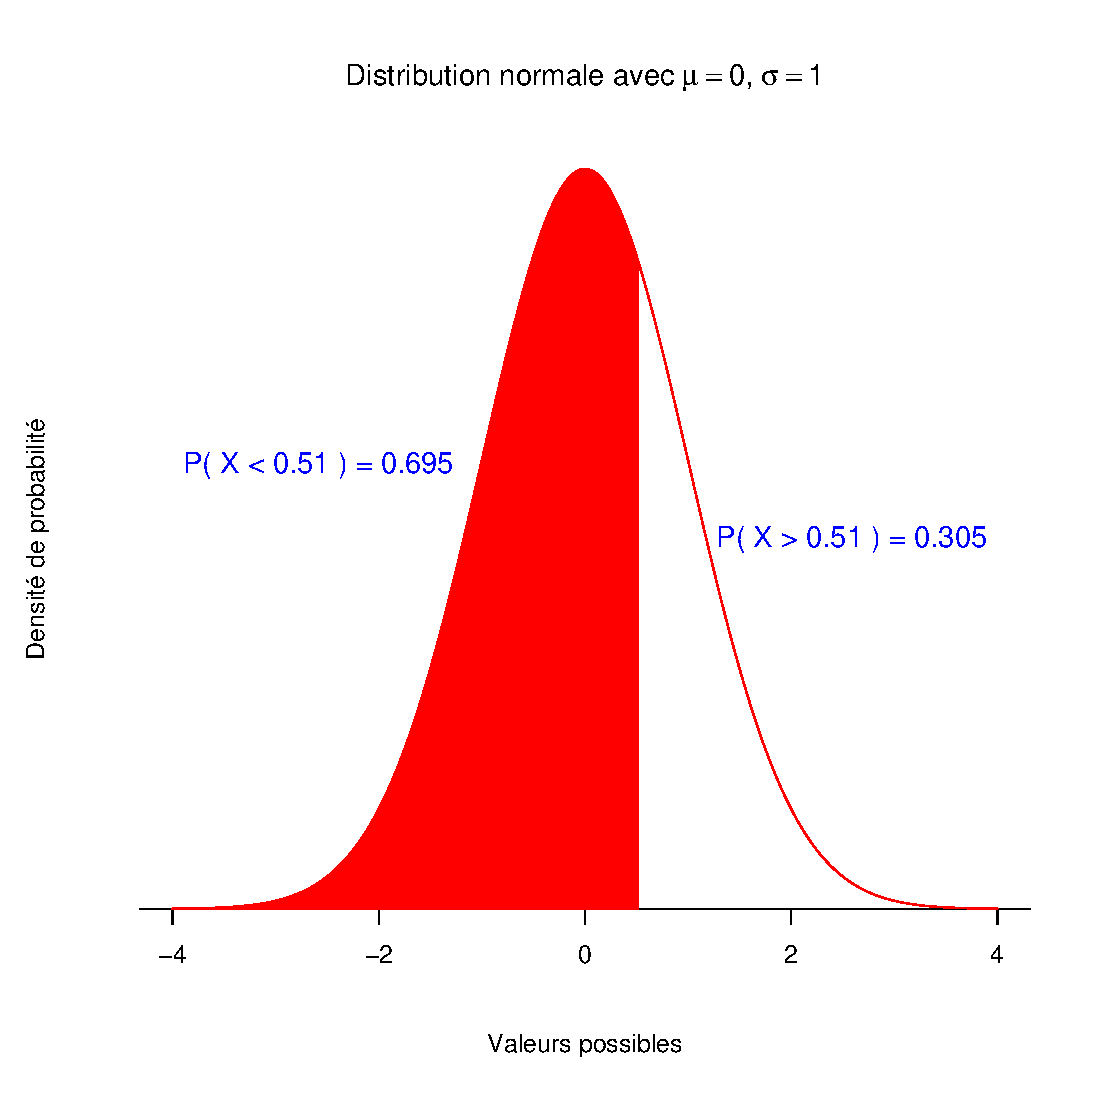
\includegraphics[scale=0.25]{norm_table}$$
%% Avec R
% x <- seq(0,3.09,by=0.01)
% z <- matrix(signif(pnorm(x),digits=4), ncol=10, byrow=TRUE, dimnames = list( seq(0,3,by=0.1), seq(0.00,0.09,by=0.01) ))
% library(Hmisc)
% latex(z, file="") # print to screen instead of write into file y.tex
{\footnotesize \input{tableNormale}}



\newpage
\section{Table de la loi du $\chi^2$}
\label{sec:tablechideux}
% \begin{center}
% \includegraphics[width=\linewidth,clip]{table_chi2}
% \end{center}
%
%% Avec R
% # Se mettre dans le bon r�pertoire
% setwd("C:/Documents and Settings/Varone/Mes documents/Cours/Stat_III/polycopie")
% # Degr�s de libert�
% dl <- c( seq(1,30,by=1),seq(40,100,by=10) )
% # Erreurs de premi�re esp�ce
% alpha <- c(0.995,0.99,0.975,0.95,0.9,0.1,0.05,0.025,0.01,0.005)
% # Fonction � utiliser pour trouver la valeur du pertile
% f <- function(dl,alpha ) round(qchisq(alpha,dl,lower.tail=FALSE),digits=4) 
% # Tableau des r�sultats
% q2 <- outer(dl,alpha,f)
% # Ent�te des lignes et colonnes du tableau de r�sultat
% dimnames(q2) <- list(dl,alpha)
% # Package pour convertir en LaTeX
% library(Hmisc)
% # Conversion en LaTeX
% latex(q2, file="tableChiCarre.tex") # print to screen instead of write into file y.tex
{\footnotesize % latex.default(q2, file = "tableq2.tex") 
%
 \begin{center}
 \begin{tabular}{l|rrrrrrrrrr}\hline
& \multicolumn{10}{c}{\bf Valeurs de $\alpha$}\\
&
\multicolumn{1}{c}{\bf 0.995}&
\multicolumn{1}{c}{\bf 0.99}&
\multicolumn{1}{c}{\bf 0.975}&
\multicolumn{1}{c}{\bf 0.95}&
\multicolumn{1}{c}{\bf 0.9}&
\multicolumn{1}{c}{\bf 0.1}&
\multicolumn{1}{c}{\bf 0.05}&
\multicolumn{1}{c}{\bf 0.025}&
\multicolumn{1}{c}{\bf 0.01}&
\multicolumn{1}{c}{\bf 0.005}\\
\hline
{\bf dl}\\
1&$ 0.0000$&$ 0.0002$&$ 0.0010$&$ 0.0039$&$ 0.0158$&$  2.7055$&$  3.8415$&$  5.0239$&$  6.6349$&$  7.8794$\\
2&$ 0.0100$&$ 0.0201$&$ 0.0506$&$ 0.1026$&$ 0.2107$&$  4.6052$&$  5.9915$&$  7.3778$&$  9.2103$&$ 10.5966$\\
3&$ 0.0717$&$ 0.1148$&$ 0.2158$&$ 0.3518$&$ 0.5844$&$  6.2514$&$  7.8147$&$  9.3484$&$ 11.3449$&$ 12.8382$\\
4&$ 0.2070$&$ 0.2971$&$ 0.4844$&$ 0.7107$&$ 1.0636$&$  7.7794$&$  9.4877$&$ 11.1433$&$ 13.2767$&$ 14.8603$\\
5&$ 0.4117$&$ 0.5543$&$ 0.8312$&$ 1.1455$&$ 1.6103$&$  9.2364$&$ 11.0705$&$ 12.8325$&$ 15.0863$&$ 16.7496$\\
6&$ 0.6757$&$ 0.8721$&$ 1.2373$&$ 1.6354$&$ 2.2041$&$ 10.6446$&$ 12.5916$&$ 14.4494$&$ 16.8119$&$ 18.5476$\\
7&$ 0.9893$&$ 1.2390$&$ 1.6899$&$ 2.1673$&$ 2.8331$&$ 12.0170$&$ 14.0671$&$ 16.0128$&$ 18.4753$&$ 20.2777$\\
8&$ 1.3444$&$ 1.6465$&$ 2.1797$&$ 2.7326$&$ 3.4895$&$ 13.3616$&$ 15.5073$&$ 17.5345$&$ 20.0902$&$ 21.9550$\\
9&$ 1.7349$&$ 2.0879$&$ 2.7004$&$ 3.3251$&$ 4.1682$&$ 14.6837$&$ 16.9190$&$ 19.0228$&$ 21.6660$&$ 23.5894$\\
10&$ 2.1559$&$ 2.5582$&$ 3.2470$&$ 3.9403$&$ 4.8652$&$ 15.9872$&$ 18.3070$&$ 20.4832$&$ 23.2093$&$ 25.1882$\\
11&$ 2.6032$&$ 3.0535$&$ 3.8157$&$ 4.5748$&$ 5.5778$&$ 17.2750$&$ 19.6751$&$ 21.9200$&$ 24.7250$&$ 26.7568$\\
12&$ 3.0738$&$ 3.5706$&$ 4.4038$&$ 5.2260$&$ 6.3038$&$ 18.5493$&$ 21.0261$&$ 23.3367$&$ 26.2170$&$ 28.2995$\\
13&$ 3.5650$&$ 4.1069$&$ 5.0088$&$ 5.8919$&$ 7.0415$&$ 19.8119$&$ 22.3620$&$ 24.7356$&$ 27.6882$&$ 29.8195$\\
14&$ 4.0747$&$ 4.6604$&$ 5.6287$&$ 6.5706$&$ 7.7895$&$ 21.0641$&$ 23.6848$&$ 26.1189$&$ 29.1412$&$ 31.3193$\\
15&$ 4.6009$&$ 5.2293$&$ 6.2621$&$ 7.2609$&$ 8.5468$&$ 22.3071$&$ 24.9958$&$ 27.4884$&$ 30.5779$&$ 32.8013$\\
16&$ 5.1422$&$ 5.8122$&$ 6.9077$&$ 7.9616$&$ 9.3122$&$ 23.5418$&$ 26.2962$&$ 28.8454$&$ 31.9999$&$ 34.2672$\\
17&$ 5.6972$&$ 6.4078$&$ 7.5642$&$ 8.6718$&$10.0852$&$ 24.7690$&$ 27.5871$&$ 30.1910$&$ 33.4087$&$ 35.7185$\\
18&$ 6.2648$&$ 7.0149$&$ 8.2307$&$ 9.3905$&$10.8649$&$ 25.9894$&$ 28.8693$&$ 31.5264$&$ 34.8053$&$ 37.1565$\\
19&$ 6.8440$&$ 7.6327$&$ 8.9065$&$10.1170$&$11.6509$&$ 27.2036$&$ 30.1435$&$ 32.8523$&$ 36.1909$&$ 38.5823$\\
20&$ 7.4338$&$ 8.2604$&$ 9.5908$&$10.8508$&$12.4426$&$ 28.4120$&$ 31.4104$&$ 34.1696$&$ 37.5662$&$ 39.9968$\\
21&$ 8.0337$&$ 8.8972$&$10.2829$&$11.5913$&$13.2396$&$ 29.6151$&$ 32.6706$&$ 35.4789$&$ 38.9322$&$ 41.4011$\\
22&$ 8.6427$&$ 9.5425$&$10.9823$&$12.3380$&$14.0415$&$ 30.8133$&$ 33.9244$&$ 36.7807$&$ 40.2894$&$ 42.7957$\\
23&$ 9.2604$&$10.1957$&$11.6886$&$13.0905$&$14.8480$&$ 32.0069$&$ 35.1725$&$ 38.0756$&$ 41.6384$&$ 44.1813$\\
24&$ 9.8862$&$10.8564$&$12.4012$&$13.8484$&$15.6587$&$ 33.1962$&$ 36.4150$&$ 39.3641$&$ 42.9798$&$ 45.5585$\\
25&$10.5197$&$11.5240$&$13.1197$&$14.6114$&$16.4734$&$ 34.3816$&$ 37.6525$&$ 40.6465$&$ 44.3141$&$ 46.9279$\\
26&$11.1602$&$12.1981$&$13.8439$&$15.3792$&$17.2919$&$ 35.5632$&$ 38.8851$&$ 41.9232$&$ 45.6417$&$ 48.2899$\\
27&$11.8076$&$12.8785$&$14.5734$&$16.1514$&$18.1139$&$ 36.7412$&$ 40.1133$&$ 43.1945$&$ 46.9629$&$ 49.6449$\\
28&$12.4613$&$13.5647$&$15.3079$&$16.9279$&$18.9392$&$ 37.9159$&$ 41.3371$&$ 44.4608$&$ 48.2782$&$ 50.9934$\\
29&$13.1211$&$14.2565$&$16.0471$&$17.7084$&$19.7677$&$ 39.0875$&$ 42.5570$&$ 45.7223$&$ 49.5879$&$ 52.3356$\\
30&$13.7867$&$14.9535$&$16.7908$&$18.4927$&$20.5992$&$ 40.2560$&$ 43.7730$&$ 46.9792$&$ 50.8922$&$ 53.6720$\\
40&$20.7065$&$22.1643$&$24.4330$&$26.5093$&$29.0505$&$ 51.8051$&$ 55.7585$&$ 59.3417$&$ 63.6907$&$ 66.7660$\\
50&$27.9907$&$29.7067$&$32.3574$&$34.7643$&$37.6886$&$ 63.1671$&$ 67.5048$&$ 71.4202$&$ 76.1539$&$ 79.4900$\\
60&$35.5345$&$37.4849$&$40.4817$&$43.1880$&$46.4589$&$ 74.3970$&$ 79.0819$&$ 83.2977$&$ 88.3794$&$ 91.9517$\\
70&$43.2752$&$45.4417$&$48.7576$&$51.7393$&$55.3289$&$ 85.5270$&$ 90.5312$&$ 95.0232$&$100.4252$&$104.2149$\\
80&$51.1719$&$53.5401$&$57.1532$&$60.3915$&$64.2778$&$ 96.5782$&$101.8795$&$106.6286$&$112.3288$&$116.3211$\\
90&$59.1963$&$61.7541$&$65.6466$&$69.1260$&$73.2911$&$107.5650$&$113.1453$&$118.1359$&$124.1163$&$128.2989$\\
100&$67.3276$&$70.0649$&$74.2219$&$77.9295$&$82.3581$&$118.4980$&$124.3421$&$129.5612$&$135.8067$&$140.1695$\\
\hline
\end{tabular}
\end{center}

}

\newpage
\section{Table de la loi de Student}
%\begin{center}
%\includegraphics[width=\linewidth,clip]{table_student}
%\end{center}
%% Avec R
% # Se mettre dans le bon r�pertoire
% setwd("C:/Documents and Settings/Varone/Mes documents/Cours/Stat_III/polycopie")
% # Degr�s de libert�
% dl <- c( seq(1,30,by=1),seq(40,100,by=10),200,500)
% # Erreurs de premi�re esp�ce
% alphaonetail <- c(0.45,0.4,0.3,0.25,0.2,0.1,0.05,0.025,0.01,0.005)
% # Fonction � utiliser pour trouver la valeur du pertile
% f <- function(dl,alphaonetail ) round(qt(alphaonetail,dl, lower.tail=FALSE),digits=4) 
% # Tableau des r�sultats
% t <- outer(dl,alphaonetail,f)
% # Ent�te des lignes et colonnes du tableau de r�sultat
% dimnames(t) <- list(dl,alphaonetail)
% # Package pour convertir en LaTeX
% library(Hmisc)
% # Conversion en LaTeX
% latex(t, file="tableStudent.tex") # print to screen instead of write into file y.tex
{\footnotesize % latex.default(t, file = "tableStudent.tex") 
%
\begin{center}
 \begin{tabular}{r|rrrrrrrrrr}
$t$ & \multicolumn{10}{c}{\bf Valeurs de $\alpha$}\\
&
\multicolumn{1}{c}{\bf 0.45}&
\multicolumn{1}{c}{\bf 0.4}&
\multicolumn{1}{c}{\bf 0.3}&
\multicolumn{1}{c}{\bf 0.25}&
\multicolumn{1}{c}{\bf 0.2}&
\multicolumn{1}{c}{\bf 0.1}&
\multicolumn{1}{c}{\bf 0.05}&
\multicolumn{1}{c}{\bf 0.025}&
\multicolumn{1}{c}{\bf 0.01}&
\multicolumn{1}{c}{\bf 0.005}\\
\hline
{\bf dl} & \\
1&$0.1584$&$0.3249$&$0.7265$&$1.0000$&$1.3764$&$3.0777$&$6.3138$&$12.7062$&$31.8205$&$63.6567$\\
2&$0.1421$&$0.2887$&$0.6172$&$0.8165$&$1.0607$&$1.8856$&$2.9200$&$ 4.3027$&$ 6.9646$&$ 9.9248$\\
3&$0.1366$&$0.2767$&$0.5844$&$0.7649$&$0.9785$&$1.6377$&$2.3534$&$ 3.1824$&$ 4.5407$&$ 5.8409$\\
4&$0.1338$&$0.2707$&$0.5686$&$0.7407$&$0.9410$&$1.5332$&$2.1318$&$ 2.7764$&$ 3.7469$&$ 4.6041$\\
5&$0.1322$&$0.2672$&$0.5594$&$0.7267$&$0.9195$&$1.4759$&$2.0150$&$ 2.5706$&$ 3.3649$&$ 4.0321$\\
6&$0.1311$&$0.2648$&$0.5534$&$0.7176$&$0.9057$&$1.4398$&$1.9432$&$ 2.4469$&$ 3.1427$&$ 3.7074$\\
7&$0.1303$&$0.2632$&$0.5491$&$0.7111$&$0.8960$&$1.4149$&$1.8946$&$ 2.3646$&$ 2.9980$&$ 3.4995$\\
8&$0.1297$&$0.2619$&$0.5459$&$0.7064$&$0.8889$&$1.3968$&$1.8595$&$ 2.3060$&$ 2.8965$&$ 3.3554$\\
9&$0.1293$&$0.2610$&$0.5435$&$0.7027$&$0.8834$&$1.3830$&$1.8331$&$ 2.2622$&$ 2.8214$&$ 3.2498$\\
10&$0.1289$&$0.2602$&$0.5415$&$0.6998$&$0.8791$&$1.3722$&$1.8125$&$ 2.2281$&$ 2.7638$&$ 3.1693$\\
11&$0.1286$&$0.2596$&$0.5399$&$0.6974$&$0.8755$&$1.3634$&$1.7959$&$ 2.2010$&$ 2.7181$&$ 3.1058$\\
12&$0.1283$&$0.2590$&$0.5386$&$0.6955$&$0.8726$&$1.3562$&$1.7823$&$ 2.1788$&$ 2.6810$&$ 3.0545$\\
13&$0.1281$&$0.2586$&$0.5375$&$0.6938$&$0.8702$&$1.3502$&$1.7709$&$ 2.1604$&$ 2.6503$&$ 3.0123$\\
14&$0.1280$&$0.2582$&$0.5366$&$0.6924$&$0.8681$&$1.3450$&$1.7613$&$ 2.1448$&$ 2.6245$&$ 2.9768$\\
15&$0.1278$&$0.2579$&$0.5357$&$0.6912$&$0.8662$&$1.3406$&$1.7531$&$ 2.1314$&$ 2.6025$&$ 2.9467$\\
16&$0.1277$&$0.2576$&$0.5350$&$0.6901$&$0.8647$&$1.3368$&$1.7459$&$ 2.1199$&$ 2.5835$&$ 2.9208$\\
17&$0.1276$&$0.2573$&$0.5344$&$0.6892$&$0.8633$&$1.3334$&$1.7396$&$ 2.1098$&$ 2.5669$&$ 2.8982$\\
18&$0.1274$&$0.2571$&$0.5338$&$0.6884$&$0.8620$&$1.3304$&$1.7341$&$ 2.1009$&$ 2.5524$&$ 2.8784$\\
19&$0.1274$&$0.2569$&$0.5333$&$0.6876$&$0.8610$&$1.3277$&$1.7291$&$ 2.0930$&$ 2.5395$&$ 2.8609$\\
20&$0.1273$&$0.2567$&$0.5329$&$0.6870$&$0.8600$&$1.3253$&$1.7247$&$ 2.0860$&$ 2.5280$&$ 2.8453$\\
21&$0.1272$&$0.2566$&$0.5325$&$0.6864$&$0.8591$&$1.3232$&$1.7207$&$ 2.0796$&$ 2.5176$&$ 2.8314$\\
22&$0.1271$&$0.2564$&$0.5321$&$0.6858$&$0.8583$&$1.3212$&$1.7171$&$ 2.0739$&$ 2.5083$&$ 2.8188$\\
23&$0.1271$&$0.2563$&$0.5317$&$0.6853$&$0.8575$&$1.3195$&$1.7139$&$ 2.0687$&$ 2.4999$&$ 2.8073$\\
24&$0.1270$&$0.2562$&$0.5314$&$0.6848$&$0.8569$&$1.3178$&$1.7109$&$ 2.0639$&$ 2.4922$&$ 2.7969$\\
25&$0.1269$&$0.2561$&$0.5312$&$0.6844$&$0.8562$&$1.3163$&$1.7081$&$ 2.0595$&$ 2.4851$&$ 2.7874$\\
26&$0.1269$&$0.2560$&$0.5309$&$0.6840$&$0.8557$&$1.3150$&$1.7056$&$ 2.0555$&$ 2.4786$&$ 2.7787$\\
27&$0.1268$&$0.2559$&$0.5306$&$0.6837$&$0.8551$&$1.3137$&$1.7033$&$ 2.0518$&$ 2.4727$&$ 2.7707$\\
28&$0.1268$&$0.2558$&$0.5304$&$0.6834$&$0.8546$&$1.3125$&$1.7011$&$ 2.0484$&$ 2.4671$&$ 2.7633$\\
29&$0.1268$&$0.2557$&$0.5302$&$0.6830$&$0.8542$&$1.3114$&$1.6991$&$ 2.0452$&$ 2.4620$&$ 2.7564$\\
30&$0.1267$&$0.2556$&$0.5300$&$0.6828$&$0.8538$&$1.3104$&$1.6973$&$ 2.0423$&$ 2.4573$&$ 2.7500$\\
40&$0.1265$&$0.2550$&$0.5286$&$0.6807$&$0.8507$&$1.3031$&$1.6839$&$ 2.0211$&$ 2.4233$&$ 2.7045$\\
50&$0.1263$&$0.2547$&$0.5278$&$0.6794$&$0.8489$&$1.2987$&$1.6759$&$ 2.0086$&$ 2.4033$&$ 2.6778$\\
60&$0.1262$&$0.2545$&$0.5272$&$0.6786$&$0.8477$&$1.2958$&$1.6706$&$ 2.0003$&$ 2.3901$&$ 2.6603$\\
70&$0.1261$&$0.2543$&$0.5268$&$0.6780$&$0.8468$&$1.2938$&$1.6669$&$ 1.9944$&$ 2.3808$&$ 2.6479$\\
80&$0.1261$&$0.2542$&$0.5265$&$0.6776$&$0.8461$&$1.2922$&$1.6641$&$ 1.9901$&$ 2.3739$&$ 2.6387$\\
90&$0.1260$&$0.2541$&$0.5263$&$0.6772$&$0.8456$&$1.2910$&$1.6620$&$ 1.9867$&$ 2.3685$&$ 2.6316$\\
100&$0.1260$&$0.2540$&$0.5261$&$0.6770$&$0.8452$&$1.2901$&$1.6602$&$ 1.9840$&$ 2.3642$&$ 2.6259$\\
200&$0.1258$&$0.2537$&$0.5252$&$0.6757$&$0.8434$&$1.2858$&$1.6525$&$ 1.9719$&$ 2.3451$&$ 2.6006$\\
500&$0.1257$&$0.2535$&$0.5247$&$0.6750$&$0.8423$&$1.2832$&$1.6479$&$ 1.9647$&$ 2.3338$&$ 2.5857$\\
$\infty$ & \multicolumn{10}{c}{cf. Distribution Normale}
\end{tabular}

\end{center}

}

% \newpage
% \section{Table de la loi de Fisher, $p$=0.95}
% \begin{center}
% \includegraphics[width=\linewidth,clip]{table_fisher_95}
% \end{center}
%
% \newpage
% \section{Table de la loi de Fisher, $p$=0.99}
% \begin{center}
% \includegraphics[width=\linewidth,clip]{table_fisher_99}
% \end{center}


%\newpage
%\section{Table du test des rangs sign�s de Wilcoxon}\label{sec:wilcoxonsigne}
%Les valeurs critiques sont donn�es par la table suivante:\\[5mm]
%%
\begin{center}
 \begin{tabular}{r|rrr}
  unilat�ral & $\alpha = 0.05$ & $\alpha = 0.025$ & $\alpha = 0.01$\\
   bilat�ral & $\alpha = 0.10$ & $\alpha = 0.05$ & $\alpha = 0.02$\\
  \hline\\
  $n$ & \multicolumn{3}{c}{Inf�rieur, Sup�rieur}\\
  \hline
  5 &  0,15 & & \\
  6 &  2,19 &  0,21 & \\
  7 &  3,25 &  2,26 &  0,28\\
  8 &  5,31 &  3,33 &  1,35\\
  9 &  8,37 &  5,40 &  3,42\\
 10 & 10,45 &  8,47 &  5,50\\
 11 & 13,53 & 10,56 &  7,59\\
 12 & 17,61 & 13,65 & 10,68\\
 13 & 21,70 & 17,74 & 12,79\\
 14 & 25,80 & 21,84 & 16,89\\
 15 & 30,90 & 25,95 & 19,101\\
 16 & 35,101 & 29,107 & 23,113\\
 17 & 41,112 & 34,119 & 27,126\\
 18 & 47,124 & 40,131 & 32,139\\
 19 & 53,137 & 46,144 & 37,153\\
 20 & 60,150 & 52,158 & 43,167
\end{tabular}
\end{center}

% \newpage
% \section{Table du test de la somme des rangs de Wilcoxon}
%$$\includegraphics[width=\linewidth,clip]{table_wilcoxon}$$


